\documentclass[aspectratio=169]{beamer}
\usetheme{Madrid}
\usepackage[utf8]{inputenc}
\usepackage[spanish,provide=*]{babel}
\usepackage{graphicx}
\usepackage{amsmath}
\usepackage{booktabs}
\usepackage{tikz}
\usetikzlibrary{arrows.meta,positioning,shapes,fit,calc}

% Tema oscuro similar a la app
\newif\iflighttheme
\lightthemetrue

\definecolor{slate900}{HTML}{0F172A}
\definecolor{slate800}{HTML}{1E293B}
\definecolor{slate700}{HTML}{334155}
\definecolor{slate200}{HTML}{E2E8F0}
\definecolor{slate100}{HTML}{F8FAFC}
% Accentos dorados/amarillos para tema ES
\definecolor{cyan400}{HTML}{FBBF24} % amber-400
\definecolor{indigo400}{HTML}{F59E0B} % amber-500 (para enlaces finos)

\iflighttheme
  \setbeamercolor{background canvas}{bg=slate100}
  \setbeamercolor{normal text}{fg=slate900}
  \setbeamercolor{frametitle}{fg=slate900,bg=slate200}
  \setbeamercolor{title}{fg=slate900}
  \setbeamercolor{subtitle}{fg=slate800}
  \setbeamercolor{structure}{fg=cyan400}
\else
  \setbeamercolor{background canvas}{bg=slate900}
  \setbeamercolor{normal text}{fg=slate100}
  \setbeamercolor{frametitle}{fg=slate100,bg=slate800}
  \setbeamercolor{title}{fg=slate100}
  \setbeamercolor{subtitle}{fg=slate100}
  \setbeamercolor{structure}{fg=cyan400}
\fi
\setbeamertemplate{navigation symbols}{}

\title{GeoAuPredict (GAP): Aprendizaje profundo para predicción geoespacial de oro}
\subtitle{Proyecto final — Curso de Deep Learning}
\author{Edward Calderón y Equipo}
\date{\today}

\begin{document}

\frame{\titlepage}

\begin{frame}{Motivación y problema}
  \begin{itemize}
    \item Relevancia: exploración, costos, riesgo.
    \item Enfoques clásicos: levantamientos, interpolación, geoestadística.
    \item Desafíos: datos heterogéneos, autocorrelación espacial, faltantes.
    \item Objetivo: aprender de datos multimodales para predecir ocurrencia de Au.
  \end{itemize}
\end{frame}

\begin{frame}{Ingesta y preprocesamiento}
  \begin{itemize}
    \item Fuentes: DEM, índices de teledetección, capas geológicas, ensayos geoquímicos, distancias a estructuras.
    \item Unificación CRS, remuestreo, recorte del área de estudio, normalización.
    \item Particiones espaciales; balance de clases.
  \end{itemize}
\end{frame}

\begin{frame}{EDA}
  \begin{itemize}
    \item Correlaciones y distribuciones; atípicos y faltantes.
    \item Mapas de ensayos y variables; clusters y hotspots.
    \item Ideas para ingeniería de características.
  \end{itemize}
\end{frame}

\begin{frame}{Flujo de la tubería}
  \centering
  \resizebox{!}{0.78\textheight}{
% Auto-generated by generate_diagrams.py
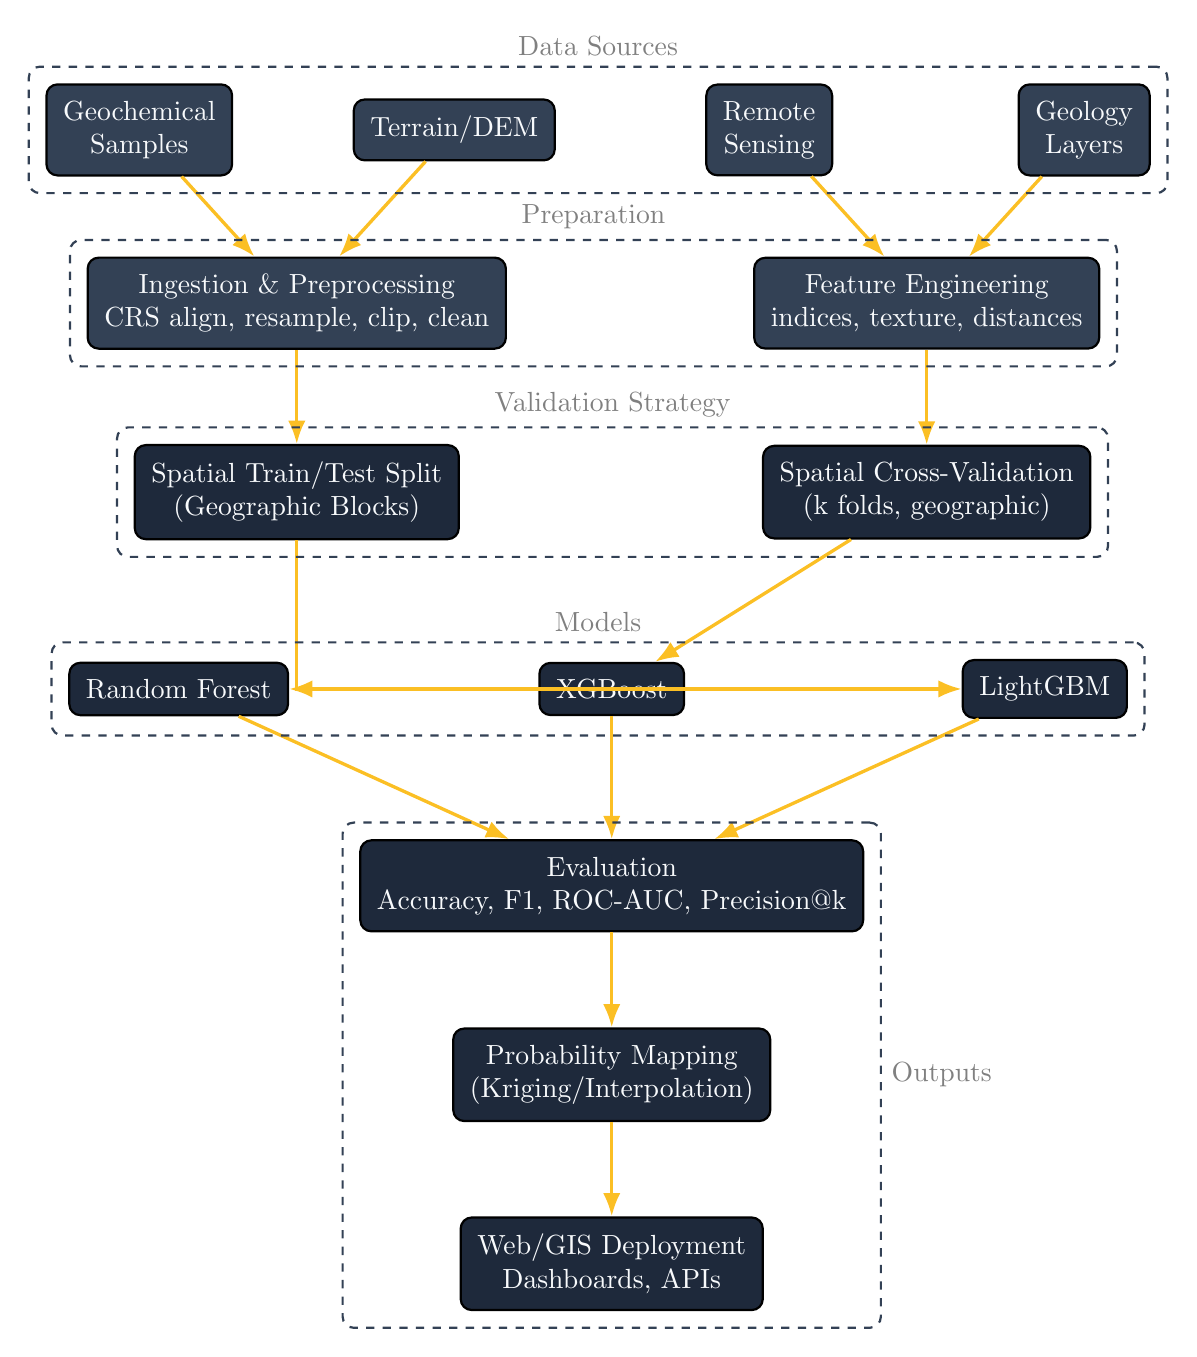
\begin{tikzpicture}[node distance=1.6cm]
  % Styles
  \tikzset{
    block/.style={draw, rounded corners, thick, align=center, fill=slate800, text=slate100, inner sep=6pt},
    data/.style={draw, rounded corners, thick, align=center, fill=slate700, text=slate100, inner sep=6pt},
    process/.style={draw, rounded corners, thick, align=center, fill=slate700, text=slate100, inner sep=6pt},
    result/.style={draw, rounded corners, thick, align=center, fill=slate800, text=slate100, inner sep=6pt},
    dashedblock/.style={draw=slate700, rounded corners, thick, align=center, dashed, inner sep=6pt},
    line/.style={-Latex, very thick, draw=cyan400},
  }

  % Row 1: Data sources (explicit coordinates to avoid overlap)
  \node[data] (geochem) at (0,0) {Geochemical\\Samples};
  \node[data] (terrain) at (4,0) {Terrain/DEM};
  \node[data] (remote)  at (8,0) {Remote\\Sensing};
  \node[data] (geology) at (12,0) {Geology\\Layers};

  % Row 2
  \node[process] (ingest) at (2,-2.2) {Ingestion \& Preprocessing\\CRS align, resample, clip, clean};
  \node[process] (feat)   at (10,-2.2) {Feature Engineering\\indices, texture, distances};

  % Row 3
  \node[block] (split) at (2,-4.6) {Spatial Train/Test Split\\(Geographic Blocks)};
  \node[block] (cv)    at (10,-4.6) {Spatial Cross-Validation\\(k folds, geographic)};

  % Row 4: Models
  \node[block] (rf)   at (0.5,-7.1) {Random Forest};
  \node[block] (xgb)  at (6.0,-7.1) {XGBoost};
  \node[block] (lgbm) at (11.5,-7.1) {LightGBM};

  % Row 5
  \node[result] (eval)    at (6.0,-9.6) {Evaluation\\Accuracy, F1, ROC-AUC, Precision@k};
  \node[result] (mapping) at (6.0,-12.0) {Probability Mapping\\(Kriging/Interpolation)};
  \node[result] (deploy)  at (6.0,-14.4) {Web/GIS Deployment\\Dashboards, APIs};

  % Edges
  \draw[line] (geochem) -- (ingest);
  \draw[line] (terrain) -- (ingest);
  \draw[line] (remote)  -- (feat);
  \draw[line] (geology) -- (feat);
  \draw[line] (ingest) -- (split);
  \draw[line] (feat)   -- (cv);
  \draw[line] (split)  |- (rf);
  \draw[line] (cv)     -- (xgb);
  \draw[line] (split)  |- (lgbm);
  \draw[line] (rf)  -- (eval);
  \draw[line] (xgb) -- (eval);
  \draw[line] (lgbm) -- (eval);
  \draw[line] (eval) -- (mapping);
  \draw[line] (mapping) -- (deploy);

  % Group boxes
  \node[dashedblock, fit=(geochem) (terrain) (remote) (geology), label={[gray]above:Data Sources}] {};
  \node[dashedblock, fit=(ingest) (feat), label={[gray]above:Preparation}] {};
  \node[dashedblock, fit=(split) (cv), label={[gray]above:Validation Strategy}] {};
  \node[dashedblock, fit=(rf) (xgb) (lgbm), label={[gray]above:Models}] {};
  \node[dashedblock, fit=(eval) (mapping) (deploy), label={[gray]right:Outputs}] {};
\end{tikzpicture}
}
\end{frame}

\begin{frame}{Enfoque de modelado}
  \begin{itemize}
    \item Ensambles: Random Forest, XGBoost, LightGBM.
    \item Validación cruzada espacial (bloques geográficos).
    \item Mapas de probabilidad e incertidumbre.
  \end{itemize}
\end{frame}

\begin{frame}{Arquitectura (Ensamble)}
  \centering
  \resizebox{\textwidth}{!}{
% Auto-generated by generate_diagrams.py
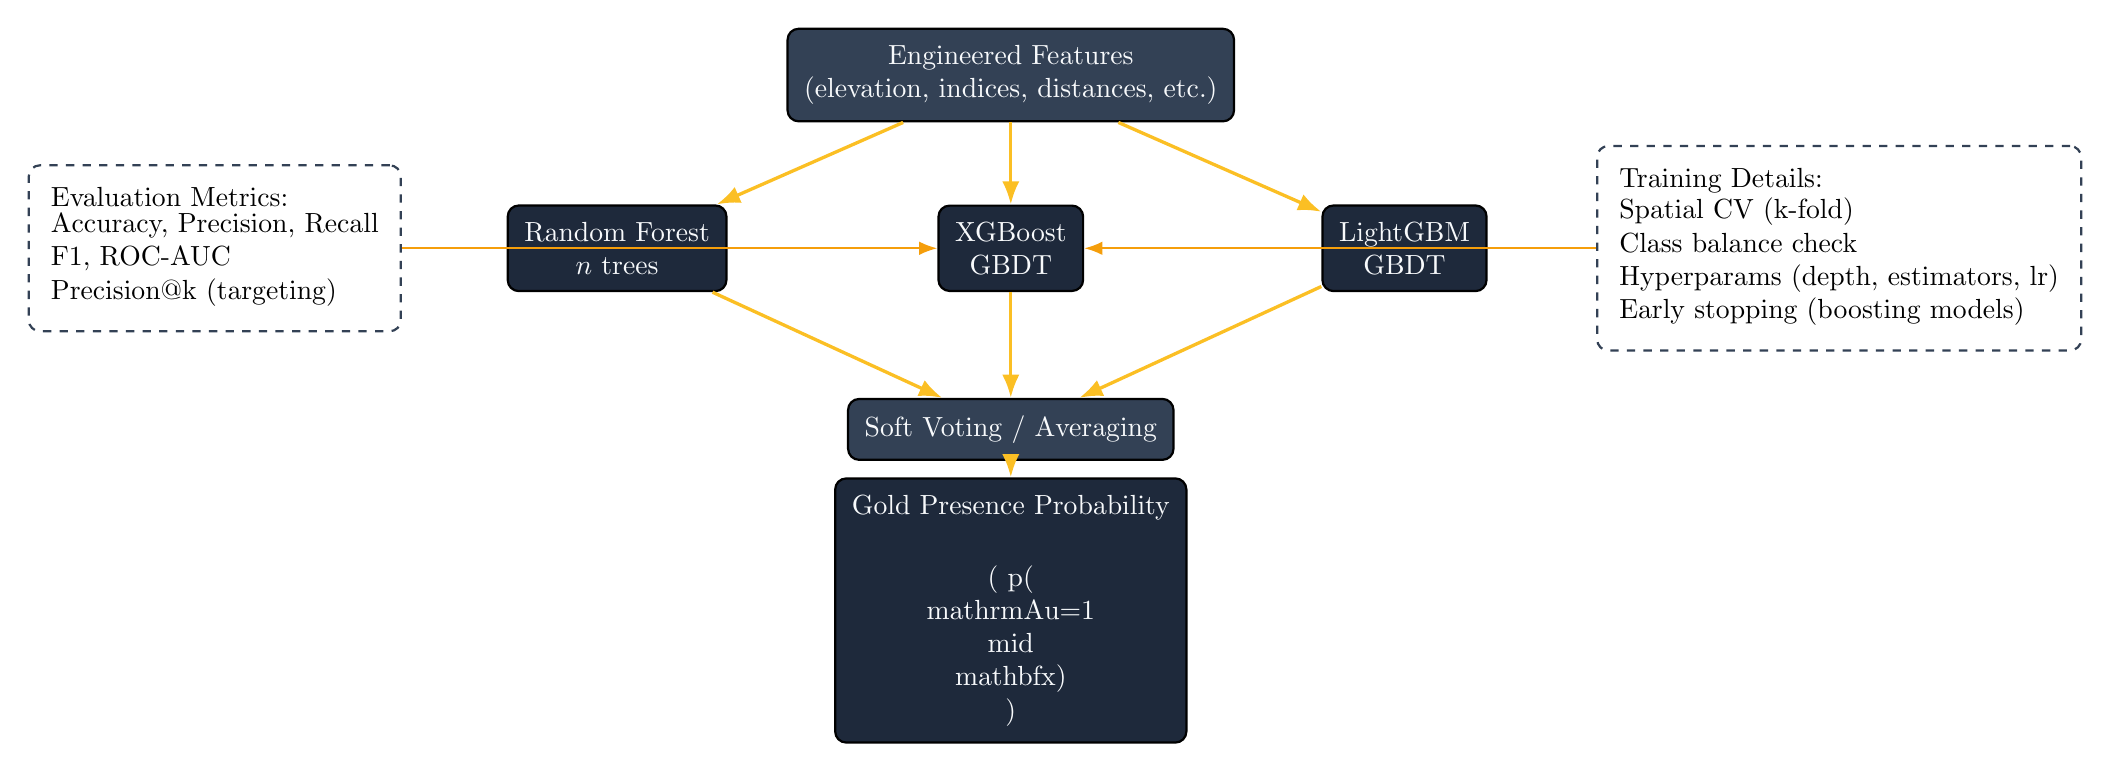
\begin{tikzpicture}[node distance=1.5cm]
  % Styles
  \tikzset{
    block/.style={draw, rounded corners, thick, align=center, fill=slate800, text=slate100, inner sep=6pt},
    data/.style={draw, rounded corners, thick, align=center, fill=slate700, text=slate100, inner sep=6pt},
    process/.style={draw, rounded corners, thick, align=center, fill=slate700, text=slate100, inner sep=6pt},
    result/.style={draw, rounded corners, thick, align=center, fill=slate800, text=slate100, inner sep=6pt},
    dashedblock/.style={draw=slate700, rounded corners, thick, align=center, dashed, inner sep=6pt},
    line/.style={-Latex, very thick, draw=cyan400},
    thinlink/.style={-Latex, thick, draw=indigo400},
  }

  % Inputs (fixed spacing)
  \node[data] (features) at (0,0) {Engineered Features\\(elevation, indices, distances, etc.)};

  % Base learners row
  \node[block] (rf)   at (-5,-2.2) {Random Forest\\$n$ trees};
  \node[block] (xgb)  at (0,-2.2)  {XGBoost\\GBDT};
  \node[block] (lgbm) at (5,-2.2)  {LightGBM\\GBDT};

  % Ensemble and output
  \node[process] (ens)  at (0,-4.5) {Soft Voting / Averaging};
  \node[result]  (proba) at (0,-6.8) {Gold Presence Probability\\[2pt] \\( p(\\mathrm{Au}=1\\mid \\mathbf{x}) \\)};

  % Links
  \draw[line] (features) -- (rf);
  \draw[line] (features) -- (xgb);
  \draw[line] (features) -- (lgbm);
  \draw[line] (rf) -- (ens);
  \draw[line] (xgb) -- (ens);
  \draw[line] (lgbm) -- (ens);
  \draw[line] (ens) -- (proba);

  % Side panels
  \node[dashedblock, right=6.5cm of xgb, align=left, inner sep=8pt] (trainbox) {Training Details:\\
    \begin{tabular}{@{}l@{}}
      Spatial CV (k-fold)\\
      Class balance check\\
      Hyperparams (depth, estimators, lr)\\
      Early stopping (boosting models)
    \end{tabular}
  };

  \node[dashedblock, left=6.8cm of xgb, align=left, inner sep=8pt] (evalbox) {Evaluation Metrics:\\
    \begin{tabular}{@{}l@{}}
      Accuracy, Precision, Recall\\
      F1, ROC-AUC\\
      Precision@k (targeting)
    \end{tabular}
  };

  \draw[thinlink] (trainbox.west) -- ++(-0.7,0) |- (xgb);
  \draw[thinlink] (evalbox.east) -- ++(0.7,0) |- (xgb);
\end{tikzpicture}
}
\end{frame}

\begin{frame}{Entrenamiento y validación}
  \begin{itemize}
    \item Métricas: Exactitud, Precisión, Recall, F1, ROC-AUC, Precision@k.
    \item Detalles: early stopping (boosting), chequeos de hiperparámetros.
    \item Resultados clave: LightGBM AUC \textbf{0.9243}; Ensamble (producción) AUC \textbf{0.9208}; AUC por bloques espaciales \textbf{0.86}.
  \end{itemize}
\end{frame}

\begin{frame}{Comparación con métodos clásicos}
  \begin{itemize}
    \item Baselines: kriging, regresión, WoE, SVM (AUC típica \(\approx 0.82\)).
    \item Mejora: +\(\sim\)\textbf{22\%} AUC (0.82 \(\to\) 0.9208/0.9243).
    \item Fortalezas: no linealidad y multimodalidad; debilidades clásicas: estacionariedad/linealidad.
  \end{itemize}
\end{frame}

\begin{frame}{Despliegue y casos de uso}
  \begin{itemize}
    \item Dashboards web, exportación GIS, APIs.
    \item Guiar muestreo, priorizar zonas, soporte a decisión.
    \item Limitaciones: shift de dominio, disponibilidad de datos, generalización.
  \end{itemize}
\end{frame}

\begin{frame}{Estrategia de Q\&A}
  \small
  \begin{tabular}{p{0.48\textwidth} p{0.48\textwidth}}
  \textbf{¿Por qué DL vs geoestadística?} & Interacciones no lineales; multimodalidad; escala. \\
  \textbf{Evitar sobreajuste} & CV espacial; regularización; early stopping; holdouts no contiguos. \\
  \textbf{Interpretabilidad} & Importancia de variables, SHAP, modelos sustitutos. \\
  \textbf{Transferencia} & Shift de dominio; fine-tuning; entrenamiento multi-región. \\
  \textbf{Incertidumbre} & MC-dropout, ensambles, regresión cuantílica (trabajo futuro). \\
  \textbf{SOTA} & Citar TorchGeo/RS DL; comparar enfoque/métricas; novedad. \\
  \textbf{Limitaciones} & Datos escasos, ruido de sensores, shift, interpretabilidad. \\
  \textbf{Operación} & Ingesta continua; inferencia; integración GIS; feedback del campo. \\
  \end{tabular}
\end{frame}

\begin{frame}{Conclusiones}
  \begin{itemize}
    \item Novedad: integración multimodal, CV espacial, mapas de probabilidad.
    \item Impacto: menores costos, mejor focalización, escalabilidad.
    \item Futuro: incertidumbre, adaptación de dominio, explicabilidad.
  \end{itemize}
\end{frame}

\begin{frame}{Preguntas}
  \centering\Large ¡Gracias!\\[0.5cm]Preguntas bienvenidas.\\[0.6cm]
  \href{https://edwardcalderon.github.io/GeoAuPredict/login}{\beamergotobutton{Demo}}\\[0.4cm]
  \small \href{https://github.com/edwardcalderon/GeoAuPredict/}{github.com/edwardcalderon/GeoAuPredict}
\end{frame}

\end{document}

